%%%%%%%%%%%%%% COPYRIGHT INFORMATION %%%%%%%%%%%%%%
% Template by
% Author: Sascha Frank 
% Nov. 2006
% University Freiburg 
% www.informatik.uni-freiburg.de/~frank/
% Distributed freely for non-commercial use

%%%%%%%%%%%%%%%%%%%%% PREAMBLE %%%%%%%%%%%%%%%%%%%%%
\documentclass{beamer}
\usepackage{beamerthemeshadow}
\usepackage{lmodern}
\usepackage{color}
\usepackage[]{url}
\usepackage{booktabs} % Allowqs the use of \toprule, \midrule and \bottomrule in tables

% include frame number on each frame
\setbeamertemplate{footline}{\quad \insertframenumber/\inserttotalframenumber}
\newcommand{\cmark}{\ding{51}} % check-mark
\newcommand{\xmark}{\ding{55}} % X-mark
\newcommand{\inv}{^{-1}}
\newcommand{\e}{\varepsilon}
\newcommand{\E}{\mathbb{E}}
\newcommand{\N}{\mathbb{N}}
\newcommand{\C}{\mathcal{C}}
\newcommand{\M}{\mathcal{M}}
\renewcommand{\P}{\mathbb{P}}
\newcommand{\R}{\mathbb{R}}
\newcommand{\Var}{\mathbb{V}}
\newcommand{\X}{\mathcal{X}}
\newcommand{\Y}{\mathcal{Y}}
\newcommand{\Z}{\mathcal{Z}}
\newcommand{\dist}{\operatorname{dist}}
\newcommand{\vi}{{\vec i}}
\newcommand{\sminus}{\backslash}

%%%%%%%%%%%%%%%%%%%%% DOCUMENT %%%%%%%%%%%%%%%%%%%%%
\begin{document}
\title{Information Theoretic Clustering using Kernel Density Estimation}
\author[Singh,Hooi]{Shashank Singh
\footnote{Machine Learning Dept. and Dept. of Statistics, \\
Carnegie Mellon University, Pittsburgh, PA, USA}
\and Bryan Hooi$^1$}
\institute{10-715 Advanced Introduction to Machine Learning}
\date{October 21, 2014}

\section{Introduction}
\frame{\titlepage}

\subsection{Background}
\frame{\frametitle{Background}
\begin{center}
\begin{itemize}
\item Between 2010-2012, several papers proposed an approach to nonparametric
clustering based on maximizing the estimated mutual information between the data points
and their labels (MIMax)
\item Steeg et al., 2014, showed that MIMax was asymptotically biased towards
clusters of equal sample size, and thus sometimes performed \emph{worse} with
more data
\end{itemize}
\end{center}
}

\frame{\frametitle{Background}
\begin{center}
\begin{itemize}
\item Intead, Steeg et al. used the axiomatic foundations of information theory
to justify an approach based on minimizing the estimated conditional entropy
$\hat H(Y | X)$ of the labels ($Y$) given the data ($X$)
\item They proposed an algorithm using a $k$-nearest neighbor estimate $\hat
H(Y | X)$
\end{itemize}
\end{center}
}

\subsection{Main Contributions}
\frame{\frametitle{Main Contributions}
Our work\ldots
\begin{itemize}
\item provides further motivation for Conditional Entropy Minimization in terms
of Minimum Description Length (MDL)
\item suggests a principled approach to determining the number of clusters
using MDL
\item provides a theoretical link between clustering CHMin and the K-means
algorithm
\item provides a novel approach to Conditional Entropy clustering via Kernel
Density Estimation (CHMin)
\item empirically compares the performance of CHMin on synthetic and real
datasets with K-means and Hierachical Clustering
\end{itemize}
}

% \frame{\frametitle{Two Papers}
% \begin{columns}[T] % align columns
% \begin{column}{.52\textwidth}
% Xing et al., 2002,
% Distance Metric Learning, with application to Clustering with side-information
% \begin{itemize}
% \item first learn metric from labeled data (``preprocessing step''), and then
% cluster
% \item single metric for all data
% \item obey all constraints
% \end{itemize}
% \end{column}%
% \hfill%
% \begin{column}{.52\textwidth}
% Bilenko et al., 2004,
% Integrating Constraints and Metric Learning in Semi-Supervised Clustering
% \begin{itemize}
% \item leverage unlabeled data for metric learning by alternating clustering and
% metric learning
% \item separate metric for each cluster
% \item soft constraints tolerate noisy supervision
% \end{itemize}
% \end{column}
% \end{columns}
% }
% 

\section{Theoretical Results}
\frame{\frametitle{Theoretical Results}
\begin{center}

{\Huge Theoretical Results}
\end{center}
}

%------------------------------------------------

\begin{frame}
\begin{itemize}
\item Principle of parsimony
\item Select the hypothesis that compresses the data the most.
\end{itemize}
\frametitle{Minimum Description Length (MDL)}
\begin{block}{Two-stage MDL}
\begin{equation*}
\underset{H}{\text{minimize}} \ \ L(H) + L(D|H)
\end{equation*}
\end{block}
\end{frame}
%-------------------------------------------------

\begin{frame}
\frametitle{Conditional Entropy Minimization and MDL}
\begin{theorem}
Under the conditions:
\begin{itemize}
\item Fixed number of clusters $K$
\item Estimate $\hat{p}$ as a mixture of a parametric distribution (e.g. mixture of Gaussians)
\end{itemize}
Minimizing description length is equivalent to minimizing estimated CE $\hat{H}(Y) + \hat{H}(X|Y)$.
\end{theorem}
\end{frame}
%----------------------------------------------------------------------------------------

\begin{frame}
\frametitle{Implications}
\begin{itemize}
\item Justifies minimizing CE
\item Can use MDL to select the number of clusters $K$
\end{itemize}
\end{frame}
%----------------------------------------------------------------------------------------

\begin{frame}
\frametitle{Selecting number of clusters using MDL}
\begin{theorem}
To select the number of clusters $K$ using MDL, we minimize
\[
\hat{H}(Y) + \hat{H}(X|Y) + \log^*(K) + Kd(\log(2B) + \frac{1}{2} \log(n)) + \log(K!)
\]
\end{theorem}
\begin{itemize}
\item Can be seen as $\hat{H}(Y) + \hat{H}(X|Y) + \text{penalty on }K$
\item Penalty grows as $O(\text{(no. of parameters)}\times \log n)$
\begin{itemize}
\item Same as BIC
\end{itemize}
\end{itemize}
\end{frame}

%------------------------------------------------

\begin{frame}
\frametitle{Conditional Entropy and the K-Means Algorithm}
\begin{theorem}
\begin{itemize}
\item Using a Gaussian kernel function $K(x) = \frac{1}{\sqrt{2\pi}} e^{\frac{-x^2}{2}}$, the estimated conditional entropy $\hat{H}(X|Y)$ satisfies:
\[ \hat{H}(X|Y) \le \log(h) + \frac{1}{2}\log(2 \pi) + \frac{1}{2h^2 n} \sum_{k=1}^K \sum_{i \in C_k} (x_i - \mu_k)^2 \]
\item Minimizing the K-means objective $\sum_{k=1}^K \sum_{i \in C_k} (x_i - \mu_k)^2$ is equivalent to minimizing an upper bound for $\hat{H}(X|Y)$.
\end{itemize}
\end{theorem}
\begin{itemize}
\item Use K-means to initialize gradient descent for conditional entropy (CE) minimization
\end{itemize}
\end{frame}

%----------------------------------------------------------------------------------------

\section{Empirical Results}
\frame{\frametitle{Empirical Results}
\begin{center}

{\Huge Empirical Results}
\end{center}
}

\subsection{Algorithms}
\frame{\frametitle{Intuition}
Why do we want to minimize
\[\frac{\hat H(Y | X)}{\hat H(Y)}?\]
\begin{itemize}
\item Points with similar $x$-values and different $y$ values increase
$\hat H(Y | X)$
\item Having a small range of $y$ values decreases $\hat H(Y)$
\end{itemize}
$\Rightarrow$ \quad minimizing the objective causes nearby $x$-values to have
similar $y$-values
}

\frame{\frametitle{CHMin: A Simple Optimization Procedure}
Want to solve:
\[\min_{y_1,\cdots,y_n \in \{0,1\}}
    \frac{\hat H(Y | X)}{\hat H(Y)}.
\]

We use gradient descent + rescaling into $[0,1]$; i.e., repeatedly:
\begin{enumerate}
\item
\[y \leftarrow y - \alpha\nabla_y \frac{\hat H(Y | X)}{\hat H(Y)}\]
\item
\[y \leftarrow \frac{y - \min_i y_i}{\max_i y_i - \min_i y_i}\]
\end{enumerate}
For $K > 2$ clusters, use soft clustering: rescale onto convex hull of
$(0,0,\cdots,0,1), (0,0,\cdots,1,0),\cdots, (1,0,\cdots,0,0)$.
}

\frame{\frametitle{CHMin: Parameter Selection}
{\bf KDE Bandwidth:} Literature suggests undersmoothing (relative to optimal
density derivative estimate). In practice, Silverman's Rule of Thumb seems to
work better than AMISE. \\

\vspace{5mm}

{\bf KDE Kernel:} We use a Gaussian kernel, but, for well-separated clusters,
bounded kernels (e.g., Epanechnikov, Uniform) work very well (converge
quickly). \\

\vspace{5mm}

{\bf Gradient Step Size:} Anything approaching $0$ slowly appears to work
($1/\log i, 1/\sqrt{i}$, etc.); affects convergence, but not final result \\

\vspace{5mm}

{\bf Initialization:} $K$-means + random restarts (1-2 seems sufficient)
}

\subsection{Synthetic Datasets}
\frame{\frametitle{Three Gaussians}
$3$ spherical Gaussians in $\R^3$
\begin{itemize}
\item Very easy data set
\end{itemize}
\begin{figure}[h!]
\centering
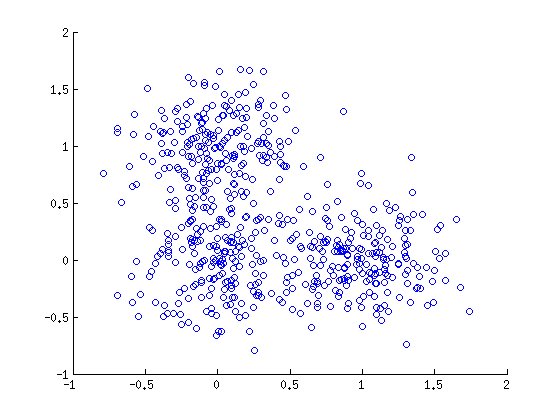
\includegraphics[width=0.7\linewidth]{3gauss}
\end{figure}
}

\frame{\frametitle{Three Gaussians}
Three clusters (chance $= 0.33$)

\vspace{15mm}
\begin{tabular}{c|c|c|c}
CHMin       & K-means++     & HC (complete) & HC (average)  \\
\hline
0.991       & {\bf 0.998}   & 0.984         & 0.994
\end{tabular}
}

\frame{\frametitle{Concentric Circles: Results}
Two concentric circles in $\R^2$
\begin{itemize}
\item Not linearly-separable
\item $2/3$ of data points in inner cluster - MIMax doesn't work well.
\end{itemize}
\begin{figure}[h!]
\centering
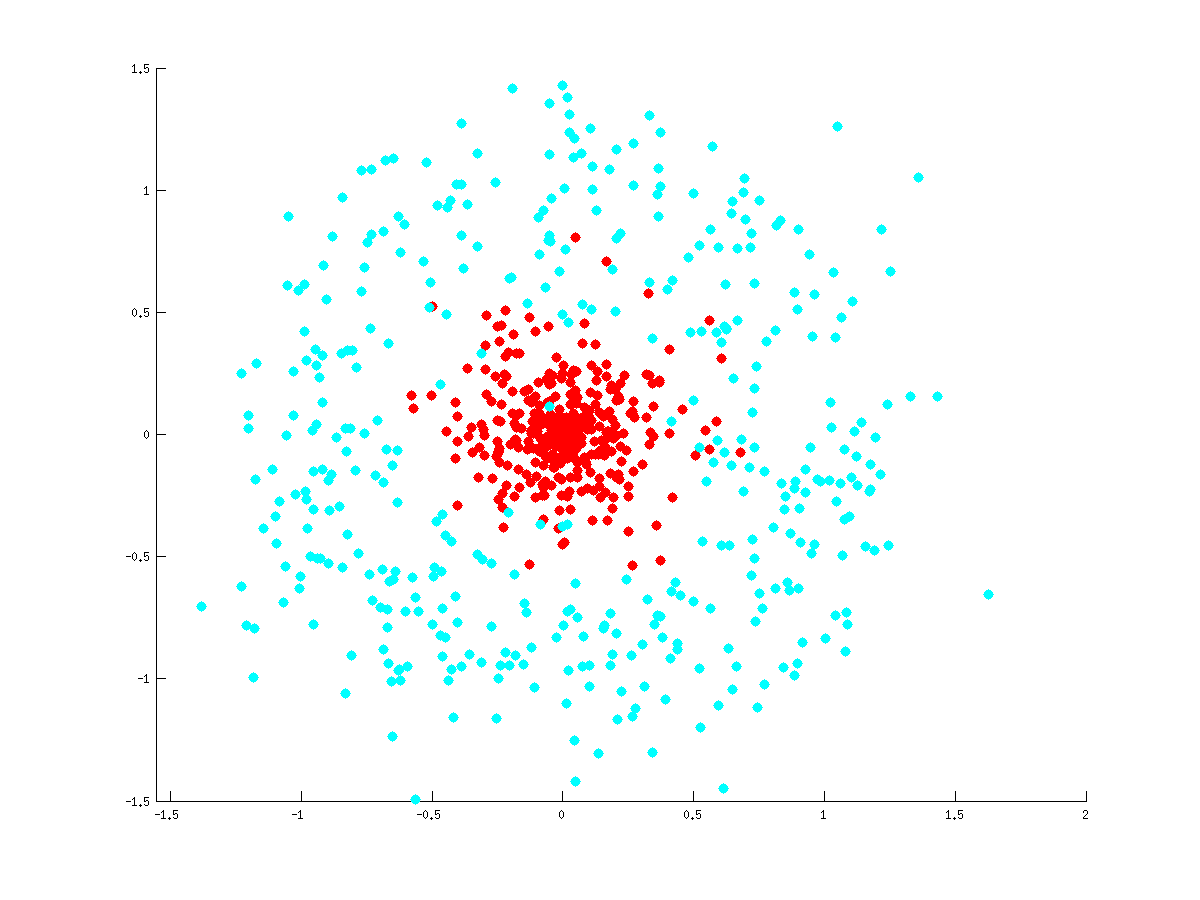
\includegraphics[width=0.7\linewidth]{con_circles_truth}
\end{figure}
}

\frame{\frametitle{Concentric Circles: Results}
Two clusters (chance $= 0.5$)

\vspace{15mm}
\begin{tabular}{c|c|c|c}
CHMin       & K-means++     & HC (complete) & HC (average)  \\
\hline
{\bf 0.894} & 0.671         & 0.677         & 0.605
\end{tabular}
}

% \frame{\frametitle{Two Bars}
% Two noisy long vertical bars in $\R^2$
% \begin{itemize}
% \item Most of variance is unrelated to clusters
% \item Normalizing only works in special (axis-parallel) cases
% \end{itemize}
% \begin{figure}[h!]
% \centering
% 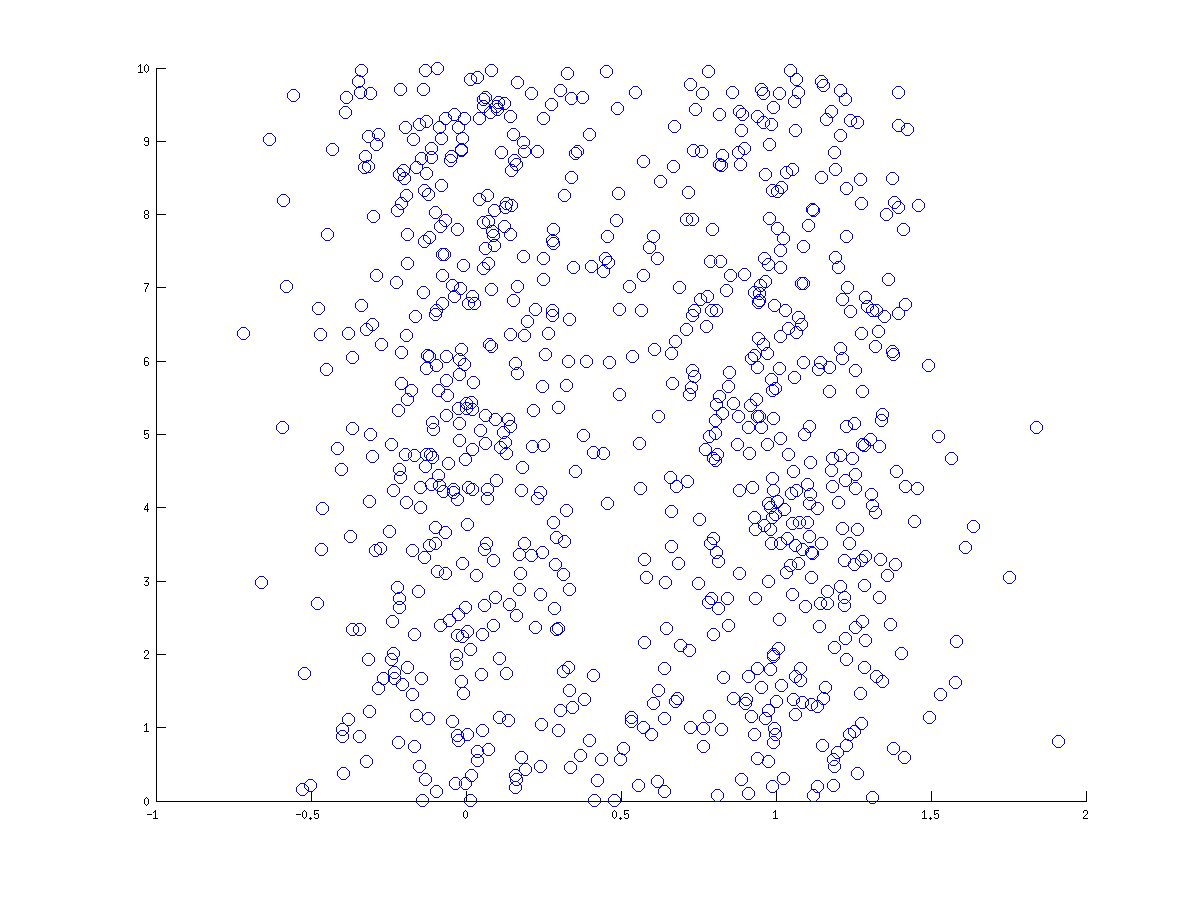
\includegraphics[width=0.7\linewidth]{two_bars}
% \end{figure}
% }
% 
% \frame{\frametitle{Two Bars: Results}
% Two clusters (chance $= 0.5$)
% 
% \vspace{15mm}
% \begin{tabular}{c|c|c|c}
% CHMin       & K-means++     & HC (complete) & HC (average)  \\
% \hline
% {\bf 0.823} & 0.520         & 0.524         & 0.524
% \end{tabular}
% }
% 
\subsection{Real Datasets}
\frame{\frametitle{Iris}
Cluster $3$ iris species using $4$ flower measurements (150 samples)
\begin{itemize}
\item One fairly distinct, linearly separable cluster.
\item Two overlapping clusters.
\item Chance $= 0.33$.
\end{itemize}
\vspace{15mm}
\begin{tabular}{c|c|c|c}
CHMin                         & K-means++     & HC (complete) & HC (average)  \\
\hline
{\bf 0.929} & 0.893         & 0.840         & 0.906         \\
\end{tabular}
}

\frame{\frametitle{Wine}
Cluster $3$ wine source using $13$ chemical properties (178 samples)
\begin{itemize}
\item One cluster is fairly distinct and linearly separable. Remaining two
overlap.
\item Chance $= 0.33$
\end{itemize}
\begin{tabular}{c|c|c|c}
CHMin                         & K-means++     & HC (complete) & HC (average)  \\
\hline
0.675       & {\bf 0.702}   & 0.674         & 0.612         \\
\end{tabular}
\begin{itemize}
\item Difficulty in high-dimensional nonparametric density estimate
\item Improved performance on (arbitrary) 5 feature subset:
\end{itemize}
\begin{tabular}{c|c|c|c}
CHMin                         & K-means++     & HC (complete) & HC (average)  \\
\hline
{\bf 0.700} & 0.494         & 0.500         & 0.500
\end{tabular}
}

\section{Conclusions}

\frame{\frametitle{Empirical Conclusions}
\begin{itemize}
\item CHMin works well on a number of (relatively small) datasets
\item Scales poorly with dimension
\begin{itemize}
\item Only depends on pairwise distances, so could combine with dimension
reduction
\end{itemize}
\end{itemize}
}

\frame{\frametitle{Future Work}
\begin{itemize}
\item Empirically, how does CHMin fare against other nonparametric clustering
approaches (e.g., MIMax, mean shift)
\item Empirically, how well does MDL identify number of clusters?
\item Can other optimization procedures speed up convergence?
\item Can we adapt error bounds from kernel density estimation?
\end{itemize}
}

\end{document}
